Created At: 2026-09-21T14:08:39-03:00
Completed At: 2026-09-21T14:08:39-03:00
File Path: `file:///home/warley/vault/research/eu/paper1_heat_burgers/paper_pinns_heat_burgers.tex`
Total Lines: 190
Total Bytes: 18954
Showing lines 1 to 190
The following code has been modified to include a line number before every line, in the format: <line_number>: <original_line>. Please note that any changes targeting the original code should remove the line number, colon, and leading space.
1: \documentclass[a4paper, 12pt, twoside]{article}
2: \usepackage{estilo}
3: 
4: % ── Margens laterais estritamente oficiais (2.5cm) conforme edital EU ──
5: \geometry{
6:   a4paper,
7:   inner=2.5cm, outer=2.5cm,
8:   top=2.0cm, bottom=1.5cm,
9:   headheight=40pt, headsep=12pt
10: }
11: \setstretch{0.86}
12: \setlength{\parindent}{0.70cm}
13: \setlength{\textfloatsep}{2pt plus 1pt minus 1pt}
14: \setlength{\intextsep}{2pt plus 1pt minus 1pt}
15: \setlength{\abovecaptionskip}{1.5pt}
16: \setlength{\belowcaptionskip}{1.5pt}
17: 
18: \title{Redes Neurais Informadas por Física para Resolução Numérica das Equações Bidimensionais do Calor e de Burgers}
19: 
20: \author{%
21:   Autor Principal\authorinfo{autor@alu.ufc.br} \\
22:   Orientador\authorinfo{orientador@ufc.br}
23: }
24: \date{}
25: 
26: \begin{document}
27: \maketitle
28: 
29: %%%%%%%%%%%%%%%%%%%%% RESUMO E ABSTRACT %%%%%%%%%%%%%%%%%%%%%%%%%%%%%%
30: 
31: \qabstract{Resumo}{Palavras-chave}{ODS}{%
32: A simulação computacional de sistemas físicos governados por Equações Diferenciais Parciais (EDPs) bidimensionais fundamenta a engenharia térmica e a fluidodinâmica. Esquemas clássicos de malha, como o Método de Diferenças Finitas (MDF) formalizado por \textcite{pereira2019}, enfrentam restrições de estabilidade (CFL) e elevado custo na discretização de geometrias complexas. Este trabalho investiga as Redes Neurais Informadas por Física (PINNs) como um paradigma contínuo e livre de malha (\textit{meshless}) na resolução de dois problemas canônicos: a Equação do Calor 2D transiente linear ($\alpha = 0{,}1$) e a Equação de Burgers 2D viscosa ($\nu = 0{,}01$) sob condição inicial quadrupolar com quatro vórtices gaussianos convergentes. As leis de conservação física são integradas ao funcional de perda multiobjetivo via diferenciação automática (\textit{autograd}) e retropropagadas para otimização dos pesos via Adam. Após 20.000 épocas, a PINN atinge resíduo $\mathcal{L}_{\mathrm{total}} = 7{,}95 \times 10^{-5}$ no calor (erro relativo $\epsilon_{L^2} = 1{,}40 \times 10^{-3}$ ou $0{,}14\%$ frente à solução analítica) e $\mathcal{L}_{\mathrm{total}} = 1{,}04 \times 10^{-3}$ em Burgers ($\mathcal{L}_{\mathrm{bc}} = 2{,}31 \times 10^{-6}$), capturando fielmente a dinâmica quadrupolar sem necessidade de malha.%
33: }{%
34: redes neurais informadas por física; equação do calor; equação de burgers; equações diferenciais parciais; diferenciação automática%
35: }{%
36: indústria, inovação e infraestrutura%
37: }
38: 
39: \qabstract{Abstract}{Keywords}{SDG}{%
40: Computational simulation of physical systems governed by two-dimensional Partial Differential Equations (PDEs) is fundamental to thermal engineering and fluid dynamics. Classical mesh-based schemes, such as the Finite Difference Method (FDM) formalized by \textcite{pereira2019}, face strict stability constraints (CFL) and high meshing overhead in complex geometries. This work investigates Physics-Informed Neural Networks (PINNs) as a continuous, mesh-free solver for two canonical problems: the linear transient 2D Heat Equation ($\alpha = 0.1$) and the nonlinear viscous 2D Burgers Equation ($\nu = 0.01$) under a quadrupolar initial condition with four converging Gaussian vortices. Physical conservation laws are directly embedded into a multi-objective loss function via automatic differentiation (\textit{autograd}) and backpropagated for weight optimization using the Adam algorithm. After 20,000 epochs, the PINN achieves residuals of $\mathcal{L}_{\mathrm{total}} = 7.95 \times 10^{-5}$ for heat (relative error $\epsilon_{L^2} = 1.40 \times 10^{-3}$ or $0.14\%$ against analytical solution) and $\mathcal{L}_{\mathrm{total}} = 1.04 \times 10^{-3}$ for Burgers ($\mathcal{L}_{\mathrm{bc}} = 2.31 \times 10^{-6}$), accurately capturing quadrupolar dynamics without meshing.%
41: }{%
42: physics-informed neural networks; heat equation; Burgers equation; partial differential equations; automatic differentiation%
43: }{%
44: industry, innovation and infrastructure%
45: }
46: 
47: %%%%%%%%%%%%%%%%%%%%%%%%%%%%%% SEÇÕES %%%%%%%%%%%%%%%%%%%%%%%%%%%%%
48: 
49: \section{Introdução}
50: 
51: A modelagem quantitativa de fenômenos de transporte térmico e dinâmica de fluidos descritos por \textbf{Equações Diferenciais Parciais (EDPs)} é indispensável no projeto de engenharia. Tradicionalmente, esquemas baseados em malha --- como o \textbf{Método de Diferenças Finitas (MDF)}, Elementos Finitos (MEF) e Volumes Finitos (MVF) --- transformam operadores diferenciais contínuos em sistemas algébricos via discretização nodal \parencite{pereira2019}. Em equações não lineares parabólicas e hiperbólicas, conforme formalizado por \textcite{pereira2019}, o MDF requer esquemas implícitos como o método ADI \parencite{peaceman1955adi} para mitigar restrições severas de estabilidade temporal ($\text{CFL} \le 1/2$), demandando malhas estruturadas e acumulando erros de truncamento local $\mathcal{O}(\Delta x^2 + \Delta t^2)$ ao longo da marcha causal.
52: 
53: Em contrapartida, as \textbf{Redes Neurais Informadas por Física (PINNs)}, introduzidas por \textcite{raissi2019pinns}, estabelecem uma abordagem contínua e livre de malha (\textit{meshless}). A solução $u_\theta(\mathbf{x}, t)$ é parametrizada por um Perceptron Multicamadas (MLP) profundo, e os operadores diferenciais são avaliados exatamente no espaço contínuo por \textbf{diferenciação automática (\textit{autograd})}. As leis físicas e condições de fronteira compõem a função de perda multiobjetivo, contornando a discretização nodal e viabilizando inferências instantâneas $\mathcal{O}(1)$.
54: 
55: Este trabalho investiga o arcabouço PINN na resolução de duas EDPs canônicas 2D: (\textit{i}) a \textbf{Equação do Calor 2D} transiente linear, validada quantitativamente frente à Série de Fourier; e (\textit{ii}) a \textbf{Equação vetorial de Burgers 2D Viscosa} sob condição inicial quadrupolar \parencite{burgers1948model, pereira2019}. Analisam-se a dinâmica de perdas, a topologia de fluxos e os ganhos de inferência contínua.
56: 
57: \section{Desenvolvimento}
58: 
59: \subsection{Fundamentação Teórica}
60: 
61: \textbf{1. Equação do Calor 2D:} A condução térmica em sólido homogêneo $\Omega = [0, 1]^2$ com difusividade $\alpha = 0{,}1\,\text{m}^2/\text{s}$ no intervalo $t \in (0, 1{,}0]\,\text{s}$ é regida por:
62: \begin{equation}
63:     \mathcal{R}_{\text{calor}}[u] := \frac{\partial u}{\partial t} - \alpha \left( \frac{\partial^2 u}{\partial x^2} + \frac{\partial^2 u}{\partial y^2} \right) = 0, \quad \forall (x, y, t) \in \Omega \times (0, 1{,}0], \label{eq:heat}
64: \end{equation}
65: sob repouso inicial $u(x, y, 0) = 0{,}0$ e contorno externo $u|_{\partial\Omega} = 1{,}0$. A solução exata analítica por separação de variáveis é a série dupla de Fourier:
66: \begin{equation}
67:     u^\star(x, y, t) = 1{,}0 - \sum_{m, n\,\text{ímp.}}^\infty \frac{16}{\pi^2 m n} \sin(m \pi x) \sin(n \pi y) e^{-\alpha \pi^2 (m^2 + n^2) t}. \label{eq:fourier}
68: \end{equation}
69: 
70: \textbf{2. Equação de Burgers 2D Viscosa:} O campo de velocidade $\mathbf{u} = [u, v]^\top$ em $\Omega = [-1, 1]^2$ com viscosidade $\nu = 0{,}01\,\text{m}^2/\text{s}$ satisfaz o sistema acoplado advectivo-difusivo \parencite{burgers1948model, pereira2019}:
71: \begin{equation}
72:     \frac{\partial u}{\partial t} + u \frac{\partial u}{\partial x} + v \frac{\partial u}{\partial y} = \nu \nabla^2 u, \quad \frac{\partial v}{\partial t} + u \frac{\partial v}{\partial x} + v \frac{\partial v}{\partial y} = \nu \nabla^2 v, \label{eq:burgers}
73: \end{equation}
74: com $\mathbf{u}|_{\partial\Omega} = \mathbf{0}$ e condição inicial quadrupolar composta por dois dipolos gaussianos ortogonais (4 vórtices convergentes ao centro):
75: \begin{equation}
76:     u_0(x, y) = e^{-10 \left[(x + 0{,}3)^2 + y^2\right]} - e^{-10 \left[(x - 0{,}3)^2 + y^2\right]}, \quad
77:     v_0(x, y) = e^{-10 \left[x^2 + (y + 0{,}3)^2\right]} - e^{-10 \left[x^2 + (y - 0{,}3)^2\right]}. \label{eq:ic_burgers}
78: \end{equation}
79: Essa configuração impõe quatro polos de velocidade de pico $\|\mathbf{u}\| \approx 1{,}0\,\text{m/s}$ orientados para a origem $(0,0)$, gerando uma zona de cisalhamento e colisão em cruz altamente desafiadora.
80: 
81: \begin{figure}[!ht]
82: \centering
83: \caption{Arquitetura e fluxo PINN: MLP profunda alimentada por coordenadas $(x,y,t)$, diferenciação automática exata via autograd e otimização multiobjetivo das perdas físicas.}
84: \label{fig:arch}
85: 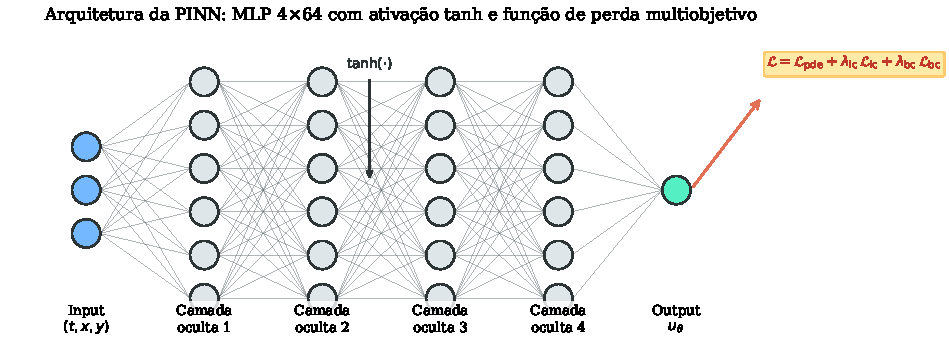
\includegraphics[width=0.64\textwidth]{figures/pinn_architecture.pdf}\\
86: {\footnotesize Fonte: Elaboração própria.}
87: \end{figure}
88: 
89: \textbf{3. Arquitetura Neural, Autograd e Retropropagação:} A aproximação contínua $\mathbf{u}_\theta(\mathbf{z})$ com entrada $\mathbf{z} = [x, y, t]^\top \in \mathbb{R}^3$ é modelada por uma MLP de $L=4$ camadas ocultas com $d_h=64$ neurônios (Figura~\ref{fig:arch}): $\mathbf{h}^{(1)} = \sigma(\mathbf{W}^{(1)}\mathbf{z} + \mathbf{b}^{(1)})$, $\mathbf{h}^{(\ell)} = \sigma(\mathbf{W}^{(\ell)}\mathbf{h}^{(\ell-1)} + \mathbf{b}^{(\ell)})$, $\mathbf{u}_\theta = \mathbf{W}^{(L+1)}\mathbf{h}^{(L)} + \mathbf{b}^{(L+1)}$, com ativação suave $\sigma(s) = \tanh(s) \in C^\infty(\mathbb{R})$. O treinamento articula um duplo fluxo de gradientes: (i) a \textbf{diferenciação automática (\textit{autograd})} em relação a $\mathbf{z}$ avalia exatamente as derivadas parciais da EDP via produtos vetor-Jacobiano (VJP): $\frac{\partial \mathbf{u}_\theta}{\partial x_j} = \nabla_{\mathbf{z}}\mathbf{u}_\theta \cdot \mathbf{e}_j$ e $\frac{\partial^2 \mathbf{u}_\theta}{\partial x_j^2} = \nabla_{\mathbf{z}}(\frac{\partial \mathbf{u}_\theta}{\partial x_j}) \cdot \mathbf{e}_j$; e (ii) o algoritmo de \textbf{retropropagação (\textit{backpropagation})} propaga o resíduo do funcional $\mathcal{L}(\theta)$ pelas camadas para computar $\nabla_\theta \mathcal{L}(\theta)$ e atualizar os pesos sinápticos via otimização estocástica.
90: 
91: \subsection{Metodologia}
92: 
93: A otimização minimiza os parâmetros $\theta$ sob o funcional multiobjetivo ponderado $L_2$:
94: \begin{equation}
95:     \mathcal{L}(\theta) = \lambda_{\mathrm{pde}}\mathcal{L}_{\mathrm{pde}}(\theta) + \lambda_{\mathrm{ic}}\mathcal{L}_{\mathrm{ic}}(\theta) + \lambda_{\mathrm{bc}}\mathcal{L}_{\mathrm{bc}}(\theta), \label{eq:loss}
96: \end{equation}
97: com $\mathcal{L}_{\mathrm{pde}} = \frac{1}{N_f}\sum \|\mathcal{R}[\mathbf{u}_\theta]\|_2^2$, $\mathcal{L}_{\mathrm{ic}} = \frac{1}{N_0}\sum \|\mathbf{u}_\theta - \mathbf{u}_0\|_2^2$, $\mathcal{L}_{\mathrm{bc}} = \frac{1}{N_b}\sum \|\mathbf{u}_\theta - \mathbf{g}\|_2^2$ e $\lambda_{\mathrm{pde}} = \lambda_{\mathrm{ic}} = \lambda_{\mathrm{bc}} = 1{,}0$. A Tabela~\ref{tab:config} sumariza os parâmetros experimentais adotados no treinamento ($20.000$ épocas Adam com $\eta = 10^{-3}$).
98: 
99: \begin{table}[!ht]
100: \centering
101: \caption{Parâmetros experimentais e hiperparâmetros de rede para Calor 2D e Burgers 2D.}
102: \label{tab:config}
103: \footnotesize
104: \setlength{\tabcolsep}{4.5pt}
105: \begin{tabular}{lcc}
106: \toprule
107: \textbf{Hiperparâmetro / Configuração} & \textbf{Equação do Calor 2D} & \textbf{Equação de Burgers 2D} \\
108: \midrule
109: Arquitetura Neural & MLP ($4 \times 64$, $\tanh$) & MLP ($4 \times 64$, $\tanh$) \\
110: Dimensão Entrada / Saída & $(x, y, t) \in \mathbb{R}^3 \to u \in \mathbb{R}$ & $(x, y, t) \in \mathbb{R}^3 \to (u, v) \in \mathbb{R}^2$ \\
111: Parâmetros Treináveis ($N_\theta$) & $12.865$ & $12.930$ \\
112: Pontos de Colocação ($N_f / N_0 / N_b$) & $10.000 \;/\; 10.000 \;/\; 4.000$ & $10.000 \;/\; 10.000 \;/\; 4.000$ \\
113: Parâmetro Físico Fundamental & $\alpha = 0{,}1\,\text{m}^2/\text{s}$ & $\nu = 0{,}01\,\text{m}^2/\text{s}$ \\
114: Domínio Espaço-Temporal & $[0, 1]^2 \times [0, 1{,}0]\,\text{s}$ & $[-1, 1]^2 \times [0, 1{,}0]\,\text{s}$ \\
115: Condição de Contorno & Dirichlet $u|_{\partial\Omega} = 1{,}0$ & Dirichlet $\mathbf{u}|_{\partial\Omega} = \mathbf{0}$ \\
116: Otimizador e Épocas & Adam ($\eta = 10^{-3}$, $20.000$ épocas) & Adam ($\eta = 10^{-3}$, $20.000$ épocas) \\
117: \bottomrule
118: \end{tabular}
119: \caption*{Fonte: Elaboração própria.}
120: \end{table}
121: 
122: \subsection{Resultados e Discussão}
123: 
124: \textbf{Dinâmica de Convergência das Perdas:} A trajetória das componentes de perda ao longo das $20.000$ iterações é apresentada na Figura~\ref{fig:loss}. No problema do calor (Figura~\ref{fig:loss}(a)), a linearidade assegura rápido decaimento assintótico, atingindo $\mathcal{L}_{\mathrm{total}} = 7{,}95 \times 10^{-5}$ com resíduo da EDP $\mathcal{L}_{\mathrm{pde}} = 6{,}47 \times 10^{-5}$. Em Burgers (Figura~\ref{fig:loss}(b)), as bordas homogêneas viabilizam $\mathcal{L}_{\mathrm{bc}} = 2{,}31 \times 10^{-6}$ e resíduo total $\mathcal{L}_{\mathrm{total}} = 1{,}04 \times 10^{-3}$, confirmando o ajuste estrito das restrições físicas.
125: 
126: \begin{figure}[!ht]
127: \centering
128: \caption{Curvas de convergência semilogarítmica do treinamento da PINN ao longo de 20.000 épocas: (a) Equação do Calor 2D ($\alpha = 0{,}1\,\mathrm{m^2/s}$); e (b) Equação de Burgers 2D ($\nu = 0{,}01\,\mathrm{m^2/s}$).}
129: \label{fig:loss}
130: 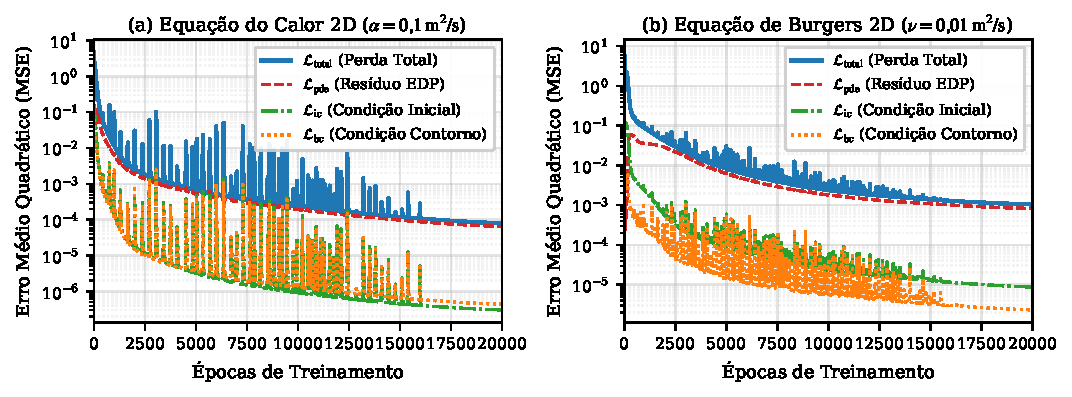
\includegraphics[width=0.92\textwidth]{figures/fig_loss_curves.pdf}\\
131: {\footnotesize Fonte: Elaboração própria.}
132: \end{figure}
133: 
134: \textbf{Experimento 1 --- Difusão Térmica 2D e Validação Analítica:} A Figura~\ref{fig:heat_3d} ilustra a evolução da superfície $u_\theta(x, y, t)$ em quatro instantes temporais. Em $t=0{,}0\,\text{s}$, a rede capta a base fria $u=0$ com contornos quentes $u=1$. Com o avanço do tempo ($t = 0{,}3 \to 0{,}7 \to 1{,}0\,\text{s}$), a difusão penetra homogeneamente ao centro. A validação frente à solução analítica em malha $100 \times 100$ comprova erro relativo $\epsilon_{L^2} = 1{,}40 \times 10^{-3}$ ($0{,}14\%$) e erro máximo $\epsilon_{L^\infty} = 1{,}29 \times 10^{-3}$.
135: 
136: \begin{figure}[!ht]
137: \centering
138: \caption{Equação do Calor 2D: evolução da distribuição de temperatura em superfície tridimensional $u_\theta(x,y,t)$ predita pela PINN para $t \in \{0{,}0;\, 0{,}3;\, 0{,}7;\, 1{,}0\}\,\mathrm{s}$ ($\alpha = 0{,}1\,\mathrm{m^2/s}$).}
139: \label{fig:heat_3d}
140: 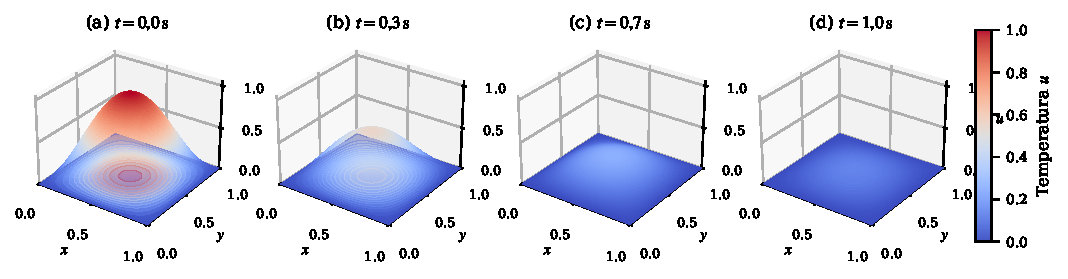
\includegraphics[width=0.88\textwidth]{figures/fig_h3_heat_3d_large.pdf}\\
141: {\footnotesize Fonte: Elaboração própria.}
142: \end{figure}
143: 
144: \textbf{Experimento 2 --- Dinâmica Não Linear dos Vórtices de Burgers 2D:} A Figura~\ref{fig:burgers} exibe a interação advectivo-difusiva da estrutura quadrupolar. Em $t=0{,}0\,\text{s}$ (Figura~\ref{fig:burgers}(a)), o campo de magnitude $\|\mathbf{u}\| = \sqrt{u^2 + v^2}$ revela quatro lóbulos simétricos de velocidade concentrados em $(\pm 0{,}3,\, 0)$ e $(0,\, \pm 0{,}3)$ com $\|\mathbf{u}\| \approx 1{,}0\,\text{m/s}$, direcionados simultaneamente para a origem. Em $t=0{,}3\,\text{s}$ (Figura~\ref{fig:burgers}(b)), a advecção não linear $(\mathbf{u}\cdot\nabla)\mathbf{u}$ atrai os quatro núcleos, deflagrando uma frente de colisão central em cruz com gradientes pronunciados. Em $t=0{,}5\,\text{s}$ (Figura~\ref{fig:burgers}(c)), ocorre a coalescência dos vórtices sob forte cisalhamento e rotação local. Em $t=1{,}0\,\text{s}$ (Figura~\ref{fig:burgers}(d)), a dissipação viscosa ($\nu = 0{,}01\,\text{m}^2/\text{s}$) amortece o fluxo para $\|\mathbf{u}\| \approx 0{,}18\,\text{m/s}$ sem gerar instabilidades numéricas.
145: 
146: \textbf{Análise Comparativa e Desempenho Computacional:} A Tabela~\ref{tab:comparison} consolida os resultados quantitativos. Enquanto esquemas clássicos de diferenças finitas investigados por \textcite{pereira2019} impõem avanços passo a passo com restrições de estabilidade CFL e interpolações nodais que degradam gradientes íngremes, a PINN resolve todo o bloco espaço-temporal $\Omega \times [0, T]$ em um bloco unificado. Uma vez ajustados os tensores $\theta$, a avaliação contínua para $10.000$ coordenadas arbitrárias em GPU requer meros $1{,}09\,\text{ms}$ no calor e $2{,}45\,\text{ms}$ em Burgers. A ativação $\tanh \in C^\infty$ permite extrair instantaneamente grandezas derivadas exatas via autograd (como fluxos térmicos $\mathbf{q} = -\kappa \nabla u$, vorticidade $\omega = \frac{\partial v}{\partial x} - \frac{\partial u}{\partial y}$ e dissipação viscosa $\varepsilon = \nu \|\nabla \mathbf{u}\|^2$) sem aproximações numéricas adicionais.
147: 
148: \begin{figure}[!t]
149: \centering
150: \caption{Equação de Burgers 2D: sequência de colisão e coalescência dos quatro vórtices gaussianos com magnitude de velocidade $\|\mathbf{u}\|$ e vetores de fluxo nos instantes $t \in \{0{,}0;\, 0{,}3;\, 0{,}5;\, 1{,}0\}\,\mathrm{s}$ ($\nu = 0{,}01\,\mathrm{m^2/s}$).}
151: \label{fig:burgers}
152: 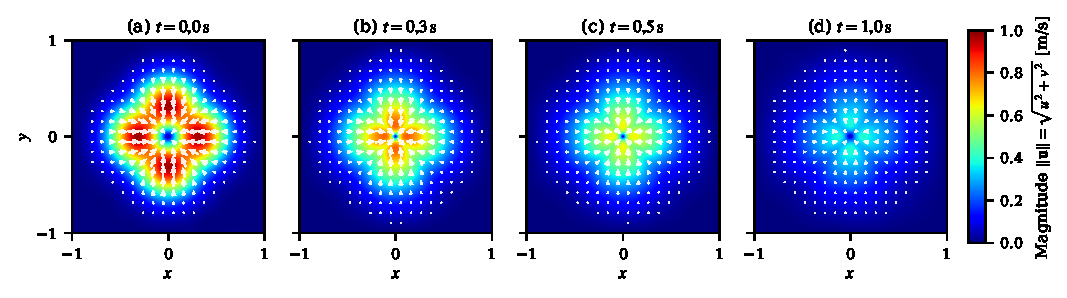
\includegraphics[width=0.88\textwidth]{figures/fig_b2_burgers_collision.pdf}\\
153: {\footnotesize Fonte: Elaboração própria.}
154: \end{figure}
155: 
156: \begin{table}[!ht]
157: \centering
158: \caption{Síntese dos indicadores quantitativos de convergência e desempenho das PINNs.}
159: \label{tab:comparison}
160: \footnotesize
161: \setlength{\tabcolsep}{3.5pt}
162: \begin{tabular}{lcc}
163: \toprule
164: \textbf{Indicador Quantitativo de Desempenho} & \textbf{Calor 2D ($\alpha = 0{,}1$)} & \textbf{Burgers 2D ($\nu = 0{,}01$)} \\
165: \midrule
166: Perda Total Final ($\mathcal{L}_{\mathrm{total}}$) & $7{,}95 \times 10^{-5}$ & $1{,}04 \times 10^{-3}$ \\
167: Resíduo da EDP ($\mathcal{L}_{\mathrm{pde}}$) & $6{,}47 \times 10^{-5}$ & $8{,}23 \times 10^{-4}$ \\
168: Resíduo de Contorno ($\mathcal{L}_{\mathrm{bc}}$) & $4{,}36 \times 10^{-7}$ & $2{,}31 \times 10^{-6}$ \\
169: Resíduo de Condição Inicial ($\mathcal{L}_{\mathrm{ic}}$) & $3{,}04 \times 10^{-7}$ & $8{,}71 \times 10^{-6}$ \\
170: Erro Relativo ($\epsilon_{L^2}$) & $1{,}40 \times 10^{-3}$ ($0{,}14\%$) & --- \\
171: Erro Máximo ($\epsilon_{L^\infty}$) & $1{,}29 \times 10^{-3}$ & --- \\
172: Tempo de Inferência ($10^4$ pontos) & $1{,}09\,\text{ms}$ & $2{,}45\,\text{ms}$ \\
173: Parâmetros / Tamanho do Modelo & $12.865$ ($198\,\text{kB}$) & $12.930$ ($202\,\text{kB}$) \\
174: \bottomrule
175: \end{tabular}
176: \caption*{Fonte: Elaboração própria.}
177: \end{table}
178: 
179: \section{Considerações Finais}
180: 
181: Os resultados comprovam que as Redes Neurais Informadas por Física constituem uma metodologia precisa, compacta e eficiente para a resolução de EDPs lineares parabólicas (Calor 2D) e sistemas acoplados fortemente não lineares (Burgers 2D). A sinergia entre o cálculo exato de operadores diferenciais via autograd e a retropropagação (\textit{backpropagation}) do funcional multiobjetivo supera os gargalos clássicos de discretização do MDF formalizados por \textcite{pereira2019}. A validação analítica comprova erro relativo inferior a $0{,}15\%$, enquanto o experimento de Burgers confirma a captura estável da dinâmica de colisão quadrupolar e amortecimento viscoso sustentada por perdas residuais $\mathcal{L}_{\mathrm{total}} \sim 10^{-3}$. O custo inicial de treinamento em GPU é amplamente amortizado pela inferência ultrarrápida em escala de milissegundos ($\sim 1 \dots 2{,}5\,\text{ms}$). Trabalhos futuros incluem problemas inversos de estimação paramétrica e escoamentos turbulentos 3D.
182: 
183: \renewcommand*{\bibfont}{\small}
184: \setlength{\bibitemsep}{2pt}
185: \begin{refcontext}[sorting=none]
186: \printbibliography
187: \end{refcontext}
188: 
189: \end{document}
190: 
The above content shows the entire, complete file contents of the requested file.
